\chapter{Model physics}\label{chap:model_physics}

\section{How to navigate this chapter}
Description of how a reader can locate the sections of particular relevance to their problem ...
perhaps a table with equation numbers and sections

\section{Underlying equations}\label{Sect:Eqns}

The state of a moving fluid can be described mathematically through means of
functions which give the distribution of velocity $\bmu=\bmu(\bmx,t)$ and
any two thermodynamics quantities (such as the pressure $p(\bmx,t)$ and
density $\rho(\bmx,t)$) within the fluid. All thermodynamic quantities are
determined by the values of any two such quantities together with the
equation of state. \citet{batchelor1967} is the ultimate reference to much of this
material. However, \cite{landau,cushman1994,panton2006,vallis2006,gill1982} are also
useful. \fluidity\ can solve the equations of motion in varying forms, and
with various approximations. These forms and approximations are discussed in
the following sections.

\subsection{Conservation equations: mass, momentum and energy}
\index{conservation!equation}
\index{momentum equation}
\index{energy equation}
A starting point for describing the physics of a continuum are the conservation equations. Fluid volumes deform in time as the fluid moves. If $\theta(\bmx,t)$ is the density of some quantity (\eg Temperature) associated with the fluid, the time evolution of that quantity in a fluid volume $V(t)$ is 
\begin{equation}\label{RTT}
 \ddt{}\left[\int_{V(t)}\theta(\bmx,t)\right]=
 \int_{V(t)}\left(\DDt{\theta}+\theta\nabla\cdot\bmu\right),
\end{equation}
\index{Reynolds Transport theorem}
which is the Reynolds' Transport theorem. In \eqref{RTT} $\bmx=(x,y,z)^T$ and $\bmu=(u,v,w)^T$ are three dimensional position and velocity vectors respectively and 
\begin{equation}\label{MatDiv}
 \DDt{}\equiv\frac{\partial}{\partial{t}}+\bmu\cdot\nabla,
\end{equation}
is the \textit{material derivative}.
\subsubsection{Mass conservation}
\index{conservation!mass}
Since matter is neither created nor destroyed, substituting $\theta=\rho$ in \eqref{RTT} gives that the \lhs\ is zero. Then, as the volume $V(t)$ is arbitrary, it is seen that the mass density satisfies
\begin{equation}\label{mass_conservation}
 \DDt{\rho}=-\rho\nabla\cdot\bmu,
\end{equation}
or equivalently
\begin{equation}\label{mass_conservation_2}
 \frac{\partial\rho}{\partial{t}}+\nabla\cdot(\rho\bmu)=0.
\end{equation}
The quantity $\rho\bmu$ is called the \textit{mass flux} or \textit{momentum} and \eqref{mass_conservation_2} is termed the \textit{equation of continuity}.

\subsubsection{Momentum conservation}
\index{conservation!momentum}
The momentum associated with a unit volume of fluid is given by $\rho\bmu$. Initially, the fluid will be considered \textit{ideal}, that is, viscosity and conductivity are assumed to be unimportant. Then, the rate of change of momentum is given by
\begin{equation}\label{mom_cons_1}
 \frac{\partial}{\partial{t}}(\rho\bmu)=\rho\frac{\partial\bmu}{\partial{t}}+\frac{\partial\rho}{\partial{t}}\bmu.
\end{equation}
Using the equation of continuity \eqref{mass_conservation_2} and Euler's
equation \citep{batchelor1967}, which is the force equation for an inviscid fluid, in the form
\begin{equation}\label{mom_cons_2}
 \frac{\partial\bmu}{\partial{t}}=-\bmu\cdot\nabla\bmu-\frac{1}{\rho}\nabla{p},
\end{equation}
gives
\begin{equation}\label{mom_cons_3}
 \frac{\partial}{\partial{t}}(\rho\bmu)=-\nabla{p}-\nabla\cdot(\rho\bmu\bmu),
\end{equation}
where $\bmu\bmu$ is a tensor which represents the dyadic product of vectors which can be written $[\bmu\bmu]_{ij}=u_{i}u_{j}$. Writing $\tensor{\Pi}=p\mathbf{I}+\rho\bmu\bmu$ \eqref{mom_cons_3} can finally be written as
\begin{equation}\label{mom_cons_4}
 \frac{\partial}{\partial{t}}(\rho\bmu)+\nabla\cdot\tensor{\Pi}=0,
\end{equation}
where $\tensor{\Pi}$ is clearly a symmetric tensor and is termed the \textit{momentum flux density tensor}.

\subsubsection{Energy conservation}
\index{conservation!energy}
The effect of energy conservation within the fluid is now considered. Consider some volume of \textit{ideal} fluid which is fixed in space such that the energy contained within this volume varies in time. The energy per unit volume of the fluid is given by
\begin{equation}\label{e_cons_1}
 \frac{1}{2}\rho{\modu}^{2}+\rho \inte,
\end{equation}
where the two terms represent the kinetic and internal energy respectively, $\inte$ being the internal energy per unit mass of the fluid. The change in energy at a fixed point in space is then given by the partial derivative of \eqref{e_cons_1} \wrt\ time
\begin{equation}\label{e_cons_2}
 \frac{\partial}{\partial{t}}\left(\frac{1}{2}\rho{\modu}^{2}+\rho\inte\right).
\end{equation}
In order to calculate this quantity the kinetic energy is first considered. Expanding the kinetic energy term of \eqref{e_cons_2} gives
\begin{equation}\label{e_cons_3}
 \frac{\partial}{\partial{t}}\left(\frac{1}{2}\rho{\modu}^{2}\right)=\frac{1}{2}\modu^{2}\frac{\partial\rho}{\partial{t}}+
                                                                 \rho\bmu\cdot\frac{\partial\bmu}{\partial{t}}.
\end{equation}
Use of \eqref{mass_conservation_2} and \eqref{mom_cons_2} gives
\begin{equation}\label{e_cons_4}
 \frac{\partial}{\partial{t}}\left(\frac{1}{2}\rho{\modu}^{2}\right)=-\frac{1}{2}{\modu}^{2}\nabla\cdot(\rho\bmu)
                                                                  -\bmu\cdot\nabla{p}
                                                                  -\rho\bmu\cdot(\bmu\cdot\nabla)\bmu.
\end{equation}
Replacing $\bmu\cdot(\bmu\cdot\nabla)\bmu$ by $\half\bmu\cdot\nabla{\modu}^{2}$ and using the thermodynamic relation for the change in heat function per unit mass of the fluid (enthalpy), $w(=\inte+p/\rho)$,  given by \citep{landau}
\begin{equation}\label{e_cons_5}
 dw=Tds+\frac{1}{\rho}dp,
\end{equation}
where $T$ is the temperature and $s$ is the entropy per unit mass, to replace $\nabla{p}$ by $\rho\nabla{w}-\rho{T}\nabla{s}$, \eqref{e_cons_4} becomes
\begin{equation}\label{e_cons_6}
 \frac{\partial}{\partial{t}}\left(\frac{1}{2}\rho{\modu}^{2}\right)=-\half{\modu}^{2}\nabla\cdot(\rho\bmu)
                                                                 -\rho\bmu\cdot\nabla\left(\half{\modu}^{2}+w\right)
                                                                 +\rho{T}\bmu\cdot\nabla{s}.
\end{equation}
It is now required to transform the derivative of the internal energy. To do this, use is made of the thermodynamic relation
\begin{equation}\label{e_cons_7}
 d\inte=Tds-pdV=Tds+(p/\rho^{2})d\rho,
\end{equation}
where $V=1/\rho$. Therefore 
\begin{equation}\label{e_cons_8}
 \frac{\partial}{\partial{t}}(\rho\inte)=w\frac{\partial\rho}{\partial{t}}+\rho{T}\frac{\partial{s}}{\partial{t}}
                                            =-w\nabla\cdot(\rho\bmu)-\rho{T}\bmu\cdot\nabla{s},
\end{equation}
where \eqref{RTT} has been used for the entropy $s$. Combining \eqref{e_cons_6} and \eqref{e_cons_8} gives
\begin{equation}\label{e_cons_9}
 \frac{\partial}{\partial{t}}\left(\half\rho{\modu}^{2}+\rho\inte\right)+\nabla\cdot\left[\rho\bmu\left(\half{\modu}^{2}+w\right)\right]=0,
\end{equation}
where $\rho\bmu\left(\half{\modu}^{2}+w\right)$ is known as the \textit{energy flux density} vector.

\subsubsection{Internal friction and thermal conduction}\label{Sect:stressed}
\index{viscosity!definition}
The effects of viscosity on the motion of a fluid are now considered. To express the equations of motion governing a viscous fluid, some additional terms are required. The equation of continuity (conservation of mass) is equally valid for any viscous as well as inviscid fluid. However, Euler's equation \eqref{mom_cons_2} and hence \eqref{mom_cons_4} and \eqref{e_cons_9} require modification.

By adding $-\tautens$ to the previously introduced \textit{momentum flux density tensor}, $\tensor{\Pi}$, so that
\begin{equation}
 \tensor{\Pi}=p\mathbf{I}+\rho\bmu\bmu-\tautens=-\sigtens+\rho\bmu\bmu,
\end{equation}
where $\sigtens=-p\mathbf{I}+\tautens$, the viscous transfer of momentum in the fluid can be taken into account. $\sigtens$ is called the stress tensor and gives the part of the momentum flux which is not due to direct transfer of momentum with the mass of the fluid. $\tautens$ is termed the viscous stress tensor. These tensors and the forms which they may take are discussed in more detail in section \ref{Sect:Rheology}. Thus, the most general form of the equations of motion of a compressible viscous fluid may be written as
\begin{equation}\label{viscous_fluids_1}
 \rho\left(\frac{\partial\bmu}{\partial{t}}+\bmu\cdot\nabla\bmu\right)=\nabla\cdot\sigtens+\rho\bmF,
\end{equation}
where $\bmF$ is the internal or volume force per unit mass (\eg gravity). The introduction of the stress tensor also modifies the form of the energy flux density. Conservation of energy of course still holds, that is: the change per unit time in the total energy of the fluid in any volume must still be equal to the total flux of energy through the surface enclosing the volume. In addition to the flux owing to the transfer of mass by the motion of the fluid, $\rho\bmu(\half{\modu}^{2}+w)$, additional terms are required. These additional terms are the flux due to processes of internal friction, $\bmu\cdot\tautens$, and the transfer of energy through \textit{thermal conduction}, denoted $\bmq$.
The complete energy flux density in a fluid with internal stress and thermal conduction therefore takes the form $\rho\bmu(\half{\modu}^{2}+w)-\bmu\cdot\tautens+\bmq$ and thus, including terms owing to volume forces $\bmF$, the general law of conservation of energy can be expressed by the equation
\begin{equation}\label{viscous_fluids_2}
 \frac{\partial}{\partial{t}}\left(\half\rho{\modu}^{2}+\rho\inte\right)
 +\nabla\cdot\left[\rho\bmu\left(\half{\modu}^{2}+w\right)-\bmu\cdot\tautens+\bmq\right]=\rho\bmF\cdot\bmu.
\end{equation}


\subsection{Compressible equations in conservative form}
Using the conservation laws outlined above the following pointwise PDE system governing the motion of a compressible fluid is obtained
% Conservation of mass, Newton's second law and the first law of
% thermodynamics allows one to derive integral relations governing the
% properties of material volumes of fluid, for background material see
% \cite{batchelor1967}. These conservation laws represent the most fundamental
% description of the properties of fluids. Since the integral relations hold
% for arbitrary volumes of fluid the following pointwise PDE system is
% obtained
\begin{subeqnarray}
\frac{\pp\rho}{\pp t} + \nabla\cdot(\rho\bmu) &=& 0,\slabel{conmass}\\
\frac{\pp}{\pp t}(\rho\bmu) + \nabla\cdot(\rho\bmu\bmu-\sigtens) &=& \rho\bmF,\slabel{conmom}\\
\frac{\pp}{\pp t}(\rho \tote) + \nabla\cdot(\rho E\bmu - \sigtens\bmu +
\bmq) &=& \rho\bmF\cdot\bmu,\slabel{conenergy}
\label{conservativesystem}
\end{subeqnarray}
where $\tote\equiv\inte+\modu^2/2$ is the total specific energy. \eqref{conmass} is exactly the conservative form of the continuity equation given in \eqref{mass_conservation_2}, \eqref{conmom} is equation \eqref{mom_cons_4} with the internal stress of the fluid and volume forces taken into account and \eqref{conenergy} is obtained from making the substitutions $w=\inte+p/\rho$ and $\tote\equiv\inte+\modu^2/2$ in \eqref{viscous_fluids_2}.

% where $\bmu$ represents the three-dimensional (3-D) velocity, $\rho$
% is the density, $\sigtens$ is a stress tensor, $\bmF$ is the
% internal or volume force per unit mass \footnote{Note that surface
% forces come in via the stress tensor.}, $\tote\equiv \inte+\bmu^2/2$ where
% $E$ is the total specific energy and $e$ is the specific internal
% energy, and $\bmq$ is the heat flux. Note that $\bmu\bmu$ represent
% the dyadic product of vectors which has components
% $[\bmu\bmu]_{ij}=\bmu_i\bmu_j$.

\subsection{Compressible equations in non-conservative form}
Expanding terms in \eqref{conservativesystem} yields the
non-conservative form of the compressible equations\footnote{\eqref{nonconmass}
is trivial to obtain. \eqref{nonconmom} makes use of \eqref{conmass}
and the divergence of the dyadic product, given by
\begin{equation*}
\nabla\cdot(\bmu\bmu) = \bmu\cdot\nabla\bmu + \bmu\nabla\cdot\bmu,
\end{equation*}
along with \eqref{MatDiv}. \eqref{nonconenergy} makes use of both \eqref{nonconmass} and \eqref{nonconmom} and
note that substituting for $\tote\equiv\inte+\modu^2/2$ results in the cancellation of kinetic energy terms.}
\begin{subeqnarray}\label{nonconform}
\DDt{\rho} + \rho\nabla\cdot\bmu &=& 0,\slabel{nonconmass}\\
\rho\DDt{\bmu} -\nabla\cdot\sigtens &=& \rho\bmF,\slabel{nonconmom}\\
\rho\DDt{\inte} - \sigtens\cdot\nabla\bmu + \nabla\cdot\bmq &=&
0.\slabel{nonconenergy} \label{nonconservativesystem}
\end{subeqnarray}
Note that, provided the fields (\eg density and pressure) vary smoothly, that is, the fields are differentiable functions, equations \eqref{conservativesystem} and \eqref{nonconservativesystem} are identical.

%The CFD code \fluidity\ can solve compressible equations in both
%conservative, non-conservative and mixed form as defined by the
%scalar BETA in $[0,1]$, in an analogous manner to theta time
%stepping defined later, \ie the weighted combination
%BETA*(\ref{conservativesystem})+($1-$BETA)*(\ref{nonconservativesystem})
%is discretised\footnote{Check that BETA and ($1-$BETA) don't need to be swapped here.}.
%This BETA has absolutely no connection with the haline contraction coefficient
%or the parameter in the beta-plane approximation.

\subsection{Some more thermodynamics and Fourier's law of heat conduction}
Classical thermodynamics \cite[Eqns (1.5.8) and (1.5.20)]{batchelor1967}
says that
\begin{equation}
T\DDt{s} = \DDt{\inte} + \frac{p}{\rho}\nabla\cdot\bmu,
\end{equation}
and
\begin{equation}
T\DDt{s} = c_p\DDt{T} -\frac{\alpha T}{\rho}\DDt{p},
\end{equation}
where $s\equiv s(p,T)$ is the entropy, $T$ is temperature, $c_p$ is
the specific heat constant $c_p=T(\pp S/\pp T)_p$, and $\alpha$ is
the thermal expansion coefficient
\begin{equation}\label{thermalexpansioncoeff}
\alpha = -\frac{1}{\rho}\frac{\pp \rho}{\pp T}.
\end{equation}

Additionally, Fourier's law states that heat flux at a point is
directly proportional to the temperature gradient there, \ie
\begin{equation}
\bmq = -\ktens\nabla T,
\end{equation}
where $\ktens$ is the coefficient of thermal conductivity in the
medium.

It is now possible to replace the internal energy equation
\eqref{nonconenergy} with a prognostic equation for temperature
\begin{equation}
\rho c_p \DDt{T} =\alpha T\DDt{p} + p\nabla\cdot\bmu
+\sigtens\cdot\nabla\bmu + \nabla\cdot(\ktens\nabla T).
\end{equation}
Messing around with the stress tensor allows one to cancel the
second term of the \rhs\ and hence
\begin{equation}
\DDt{T} =\frac{\alpha T}{\rho c_p}\DDt{p} +
\frac{\Phi}{c_p} + \nabla\cdot(\kaptens\nabla T),
\end{equation}
where $\kaptens = \ktens/(\rho c_p)$ is the heat diffusivity tensor
and
\begin{equation}
\Phi \equiv \frac{2\mu}{\rho}\left(\strt_{ij}\strt_{ij}
-\frac{1}{3}(\nabla\cdot\bmu)^2\right),
\end{equation}
is the rate of dissipation of mechanical energy, per unit mass, due
to viscous effects, see \cite[Sections 3.4 and 3.6]{batchelor1967}. This term corresponds
to the generation of heat by viscous damping, and in the sequel shall be assumed to
be of negligible importance.

\subsection{Scalar equations}
The general form the equation that governs the evolution of a scalar fields $c$
(\eg passive tracer, species concentration, temperature, salinity) is
\begin{equation}\label{eq:general_scalar_eqn}
\ppt{c} + \nabla\cdot(\bmu c) = \nabla\cdot(\kaptens\nabla c) - \sigma c + F.
\end{equation}

\subsubsection{Advection}
The advection term in \eqref{eq:general_scalar_eqn} expresses the transport of 
the scalar quantity $c$ with the flow field $\bmu$. The term convection is often
used for this process where the motion is largely vertical and as the results of
temperature (density) differences.
The advection term in \eqref{eq:general_scalar_eqn} may be written
\begin{equation}\label{eq:scalar_advection}
\nabla\cdot(\bmu c) = \bmu\cdot\nabla c + (\nabla\cdot\bmu)c.
\end{equation}
Note that for incompressible flow the second term on the \rhs\ is zero. However, there may be numerical
reasons why the discrete velocity field is not exactly divergence free, in which case this term may
be included in the discretisation, see section \ref{sect:??}. Note also that the second term on
the \rhs\ of \eqref{eq:scalar_advection} may be interpreted as a source term for $c$.

\subsubsection{Diffusion}
The diffusion term in \eqref{eq:general_scalar_eqn} represents the mixing of $c$ and may be due to 
molecular mixing of individual particles via Brownian motion, or mixing via large (compared to the
molecular scale) eddies in the flow.
The diffusion term
\begin{equation}\label{eq:scalar_diffusion}
\nabla\cdot(\kaptens\nabla c),
\end{equation}
takes some convenient simpler forms for tensor diffusivities often encountered. Often an
isotropic diffusivity, $\kaptens = \mathrm{diag}(\kappa,\kappa,\kappa)$ in which case the diffusion term
may be written as
\begin{equation}\label{eq:scalar_isotropic_diffusion}
\nabla\cdot(\kaptens\nabla c) = \kappa\nabla\cdot\nabla c = \kappa\nabla^2 c = \kappa\Delta c.
\end{equation}
In domains with high aspect ratio dynamics one often uses a smaller value of diffusivity in the `thin'
direction. For example, in the atmosphere or ocean we may choose a horizontal diffusivity $\kappa_H$ and a
vertical diffusivity $\kappa_V$ so that
$\kaptens = \mathrm{diag}(\kappa_H,\kappa_H,\kappa_V)$ with $\kappa_V < \kappa_H$ and. 
In this case the diffusion term may be written as
\begin{equation}\label{eq:scalar_isotropic_diffusion}
\nabla\cdot(\kaptens\nabla c) = \kappa_H \left(\pptt[x]{c} + \pptt[y]{c}\right) + \kappa_V \pptt[z]{c}.
\end{equation}
Note that this second order term is often termed Laplacian diffusion, the 4th order version is sometimes
termed hyper-diffusion. Hyper-diffusion acts in a similar manner to Laplacian diffusion but is more
scale selective.

\subsubsection{Absorption}
The absorption term in \eqref{eq:general_scalar_eqn} 
\begin{equation}\label{eq:scalar_absorption}
-\sigma c,
\end{equation}
has the effect of decreasing the magnitude of $c$ (note the minus sign and the fact 
that $\sigma$ would typically be positive. It is sometimes termed Rayleigh friction. 

\subsubsection{Reaction and source}
The remaining term in \eqref{eq:general_scalar_eqn}
\begin{equation}\label{eq:scalar_source}
F = \sum_i F_i,
\end{equation}
can encompasses a number of source and reaction terms. Those terms where $F_i$ are
a given function of time, location or a-priori known fields are termed sources (and sometime
sinks if they are negative). Those terms which are also functions of other prognostic fields
are termed reactions and are common when dealing with chemistry or biology.



\section{Extensions, assumptions and derived equation sets}\label{sect:eqn_extensions}
Under certain conditions, the equations of Section \ref{Sect:Eqns} can be simplified according to various approximations. In this section we derive the approximate forms of the conservation equations that are appropriate for different problems. 

\subsection{Incompressibility} \label{sect:incompressibility}
A number of assumptions lead to the consideration of an incompressible fluid or flow (see section \ref{sect:equation_of_state}). In this case one replaces the continuity equation \eqref{nonconmass} with:
\begin{equation}\label{eq:divfree}
\nabla\cdot\bmu=0.
\end{equation}
This has the effect of changing mass conservation to volume conservation.

\subsection{The anelastic approximation}
\index{sound waves}
The mass conservation equation \eqref{nonconmass} supports sound waves, but sound waves have no direct influence on most forms of convection / motion. Analytic simplicity can often be achieved by approximating the governing equations with alternative sets of filtered equations, that do not support sound waves. From a numerical perspective, eliminating sound waves may also allow the resulting system of equations to be numerically integrated using a much larger time-step than would be possible with the original un-filtered equations. 

To filter sound waves from the governing equations, it is necessary to sever the link between density perturbations and pressure perturbations. This can be accomplished through any of a family of related approximations that neglect terms involving the time variation of the density in the mass continuity equation \eqref{nonconmass}.

One approximation that will filter sound waves is obtained by assuming that the flow is incompressible (see sections \ref{sect:incompressibility} and \ref{sect:equation_of_state}), in which case the continuity equation \eqref{nonconmass} is replaced with \eqref{eq:divfree}. As noted previously, this has the effect of changing mass conservation to volume conservation. The approximation of \eqref{nonconmass} by \eqref{eq:divfree} is widely referred to as the \textit{Boussinesq approximation}. Unfortunately, the term `Boussinesq approximation' has been used in two different senses. In some disciplines, the Boussinesq approximation refers only to the approximation of mass conservation by volume conservation. However, the Boussinesq approximation traditionally includes both the preceding and additional approximations in the momentum equation. The latter definition appears to be consistent with the actual approximations employed by Boussinesq and will be the form of the Boussinesq approximation described in Section \ref{sect:boussinesq_approximation}.

A second approximation to the full compressible continuity equation is \textit{anelastic compressibility} \citep{ogura62}:
\begin{equation}\label{eq:anelastic}
\nabla\cdot (\rho_{0} \bmu) = 0. 
\end{equation}
\index{density!reference}
in which the density involved in the mass budget is a steady reference-state density $\rho_{0}(z)$ that varies only along the coordinate axis parallel to the gravitational restoring force. Such an approximation is valid if (and only if!) variations in density (for example those arising from thermal expansion) are small compared to the reference density:
\begin{equation}\label{eq:densref}
\rho(\bmx,t) = \rho_0 + \rho'(\bmx,t),\qquad \rho'\ll\rho_0.
\end{equation}

\subsection{The Boussinesq approximation} \label{sect:boussinesq_approximation}
\index{density!reference}
\index{Boussinesq!approximation}
As noted in the previous section, for many problems, one is able to assume that density does not vary greatly about a mean reference state \eqref{eq:densref}. The Boussinesq approximation involves two steps. The first makes use of this assumption in \eqref{nonconmass}, yielding \eqref{eq:divfree} --- mass conservation thus becomes volume conservation and sound waves are filtered. The second part of the Boussinesq approximation follows by replacing $\rho$ by $\rho_0$ in all terms of \eqref{nonconmom}, except where density is multiplied by gravity (i.e. in the buoyancy term where full density must be retained --- these are the density variations that drive natural convection). This yields
\begin{equation}
\rho_0\DDt{\bmu} -\nabla\cdot\sigtens = -\rho g\bmk +
\rho_0\bmF,
\end{equation}
where buoyancy has explicitly been removed from the forcing term $\bmF$.

\subsection{The non-hydrostatic Boussinesq equations}\label{sect:typical_ICOM_equations}
\index{Boussinesq!equations}
\index{momentum equation}
\index{continuity equation}
Combining the various steps above yields the three-dimensional
non-hydrostatic Boussinesq equations, as follows, which are
discretised in a domain $\Omega\subset\mathbb{R}^3$ to yield a
finite element numerical ocean model,
%
\begin{subeqnarray}
\frac{\pp\bmu}{\pp t} + (\bmu -\hat{\bmu})\cdot\nabla \bmu + 2 \bmOmega \times \bmu
&=& - \nabla p - g\nabla\eta - \rho g \bmk + \nabla\cdot \tautens + \bmF,
\slabel{mtm}\\
\nabla\cdot {\bmu}&=&0,\slabel{conty}\\
\frac{\pp T}{\pp t} + (\bmu-\hat{\bmu})\cdot\nabla  T  &=&
\nabla . \left ( \kaptens_T  \nabla T\right),\slabel{heat}\\
\frac{\pp S}{\pp t} + (\bmu-\hat{\bmu})\cdot\nabla  S  &=&
\nabla . \left ( \kaptens_S  \nabla S\right),\slabel{salt}\\
\rho &=& -\alpha(T-T_0)+\beta (S-S_0).\slabel{state}
\label{boussinesq}
\end{subeqnarray}
%
Here, $\bmu$ is the three-dimensional velocity vector,
$\hat{\bmu}$ is a term used to account for a moving reference
frame, for example in this work it takes the form of node velocities
for numerical discretisations on moving meshes (\eg to account for a moving free surface).
$t$ represents time, $p$ is the
perturbation pressure, $g$ is the acceleration due to gravity,
$\rho$ is the perturbation density,
$T$ is the temperature and $S$ is salinity. In this work $T,S$ and hence $\rho$ are all
constant. $\eta$ is the free surface height, whose evolution is described in a section below.
$\tautens,\kaptens_T,\kaptens_S$ are the viscosity, thermal diffusivity and saline
diffusivity tensors respectively. $\alpha$ is the thermal expansion coefficient
and $\beta$ is the saline contraction coefficient.
The rotation vector is $\bmOmega$, and $\bmF$ contains additional source terms such as the astronomical tidal forcing.

\subsection{Stokes flow}\label{stokesflow}
To quantify the relative sizes of inertial and viscous terms, we introduce the idea of scales of variation. Let $U_{0}$ be a typical value of $\mathbf{u}$ and let $L$ be a typical length scale on which $\mathbf{u}$ is varying. Comparing inertial and viscous terms:
\begin{equation}
\frac{\parallel \rho \mathbf{u} \cdot \nabla \mathbf{u} \parallel}{\parallel \mu \nabla^{2} \mathbf{u} \parallel} \simeq \frac{\rho U_{0}^{2} / L}{\mu U_{0} / L^{2}} = \frac{U_{0} L}{\nu} = \Re
\end{equation}
where $\Re$ is the Reynolds number of the flow. It is clear that there is
some flexibility about the choice of $U_{0}$ and $L$ and hence the precise
definition of $\Re$. However, if the Reynolds number is high ($\Re \gg 1$)
viscous forces may be negligible, whereas at low Reynolds number ($\Re \ll 1$)
the non-linear inertial forces may be ignored. This is the limit considered
in this section.

\subsubsection{The Stokes equations}
\index{Stokes equations}
In this case, $\Re \ll 1$ and we neglect inertial terms in the Navier-Stokes equations \eqref{??} to obtain:
\begin{subeqnarray}
\mu \nabla^{2} \mathbf{u} - \nabla P + \mathbf{F} = 0, \slabel{stokes_mom} \\
\nabla \cdot \mathbf{u} = 0.\slabel{stokes_mass} \label{stokessystem}
\end{subeqnarray}
These are the (forced) Stokes equations. There are no time derivatives in \eqref{stokessystem}. Thus $\mathbf{u}$ responds instantaneously to the force $\mathbf{F}$ or boundary conditions. For instance, a sphere falling in an unbounded fluid achieves its terminal velocity at once. Equation \eqref{stokes_mom} is also linear (there is no $\mathbf{u} \cdot \nabla \mathbf{u}$ term). 

\subsection{Equations in a moving reference frame}\label{sect:coriolis}
\index{Coriolis}
Newton's second law holds in a fixed inertial reference frame, \ie
fixed with respect to the distant stars. 
Examples of systems which one may wish to study with boundaries moving
with respect to this fixed inertial frame include translating and spinning tanks
and the rotating Earth. For these systems it is often convenient to rewrite the 
underlying equations within the moving frame. Extra terms then need to be considered 
which account for the fact that the acceleration of a fluid parcel relative to the 
moving reference frame is different to the acceleration with respect to the fixed 
inertial frame, and the latter is the one which allows us to invoke Newton's Laws.
For useful discussions see \citep{batchelor1967,cushman1994,knauss,vallis2006,gill1982}.

\begin{figure}\label{fig:rotating_frame}
\centering
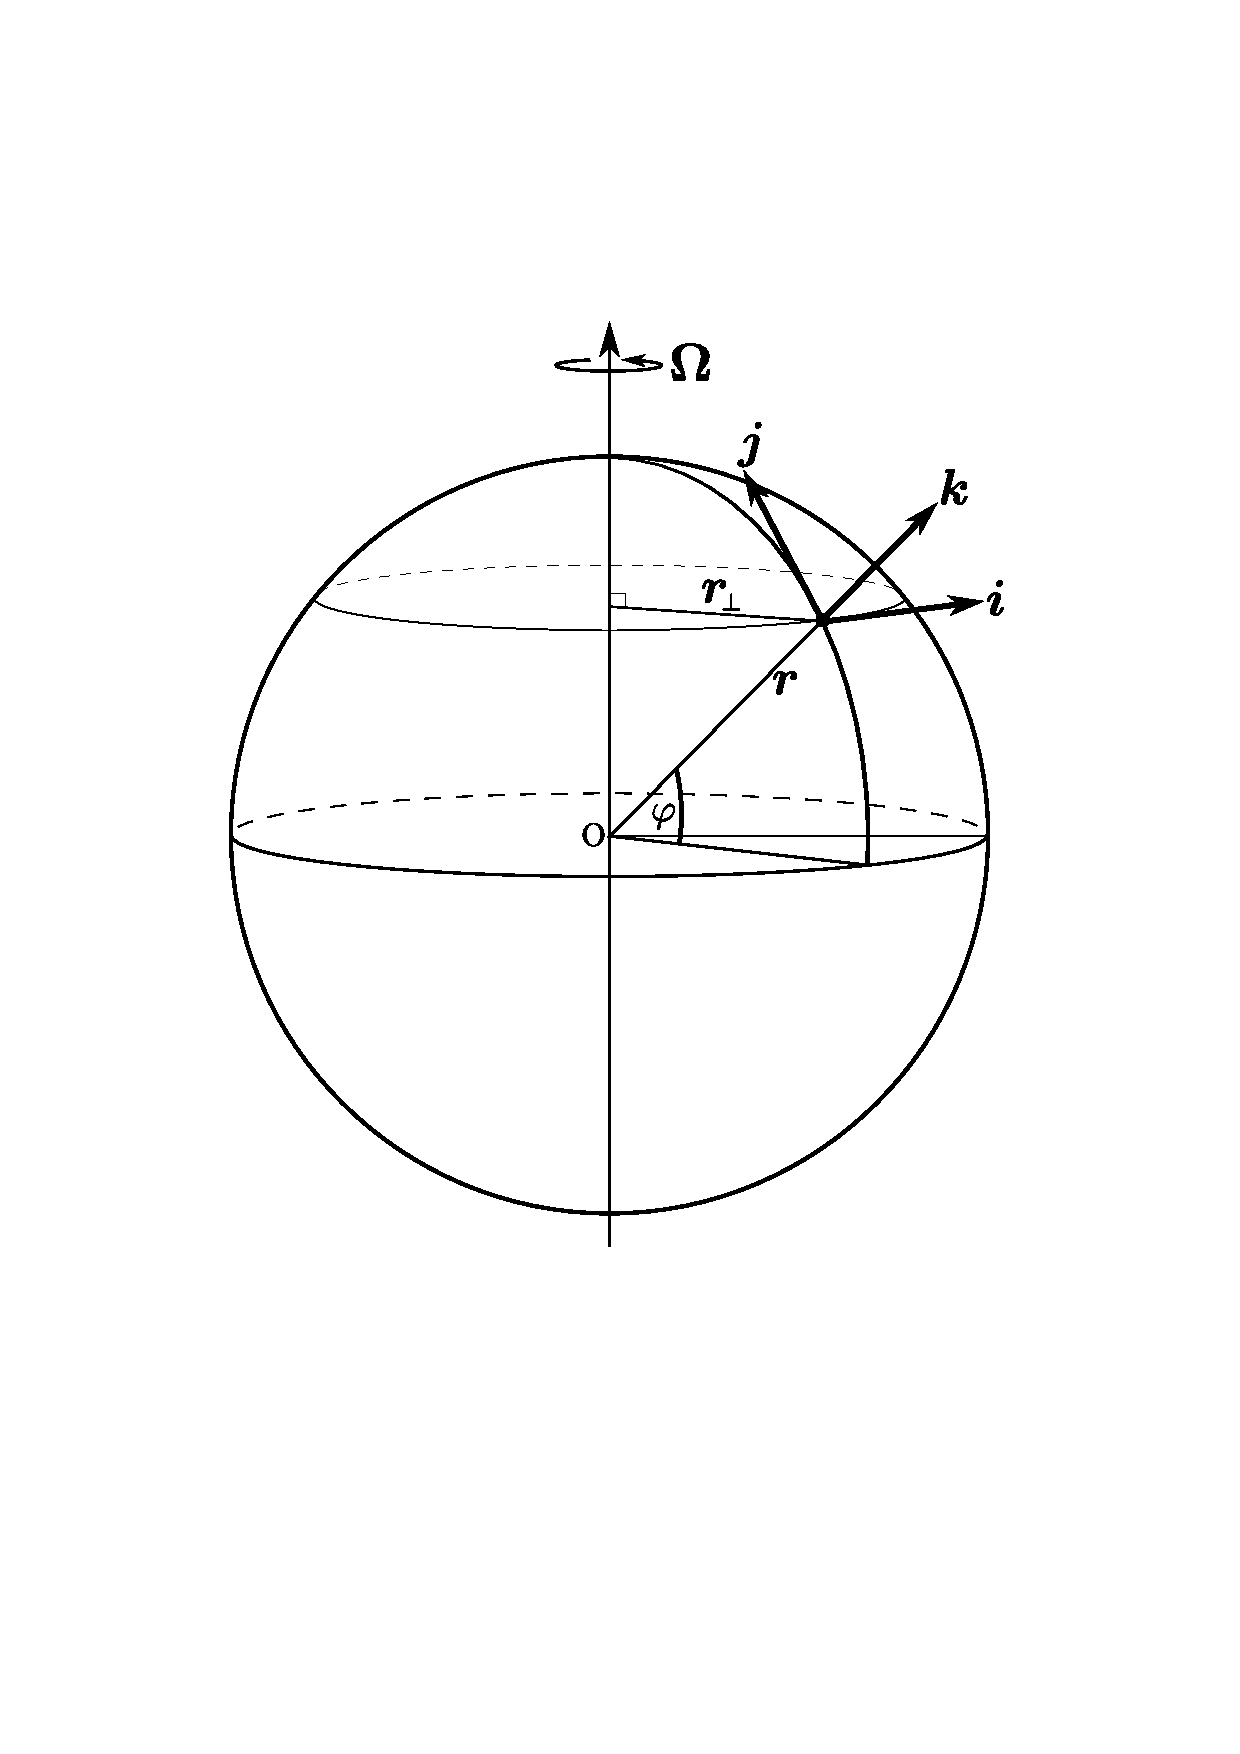
\includegraphics[width=8.0cm]{misc_images/coordinates.pdf}
\caption{Schematic of coordinates in a frame rotating with a sphere. The rotation is about a vector
pointing from South to North pole. A point on the surface of the sphere $\bmx$ and its perpendicular
distance from the axes of rotation $\bmx_{\perp}$ are shown. The latitude of $\bmx$ is given by $\phi$ 
and the unit vectors $\bmi$, $\bmj$ and $\bmk$ represent a local coordinate axes at point $\bmx$ in the rotating
frame: $\bmi$ points Eastwards, $\bmj$ points Northwards and $\bmk$ points in the radial outwards direction.}
\end{figure}

Consider a point
\begin{equation*}
\bmr = x\bmi + y\bmj + z\bmk,
\end{equation*}
where $\bmi,\,\bmj,\,\bmk$ represent axes in a coordinate system in the moving frame of
reference, \eg pointing East, North and upwards at a particular point on the Earth's surface.
The rate of change of point $\bmr$ with time in the inertial frame can then be written
\begin{equation*}
\left(\ddt{\bmr}\right)_i=\left(\ddt{x}\bmi+\ddt{y}\bmj+\ddt{z}\bmk\right)
+\left(x\ddt{\bmi}+y\ddt{\bmj}+z\ddt{\bmk}\right).
\end{equation*}
The first term on the \rhs\ is the rate of change of the point as it appears
to an observer in the moving reference frame and which can be denoted by
$(\d\bmr/\d t)_r=\bmu_r$.
The second term on the \rhs\ accounts for the movement of the reference coordinate system
with respect to the fixed inertial frame. The case or a rotating reference frame is now considered,
the translational case is simpler and follows by analogy. Suppose the moving reference frame is
rotating with an angular velocity $\bmOmega$, then the second term above can be written $\bmOmega\times\bmr$.
Hence, we may write $\bmu_i=\bmu_r+\bmOmega\times\bmr$.

This procedure can be repeated to consider rates of change of velocity, \ie accelerations. This can be most
easily achieved by noting that the time derivatives in the two reference frames are related via
\begin{equation*}
\left(\ddt{}\right)_i=\left(\ddt{}\right)_r + \bmOmega\times,
\end{equation*}
and so 
\begin{eqnarray*}
\bma_i=\left(\ddt{}\right)_i\bmu_i &=& \left(\left(\ddt{}\right)_r + \bmOmega\times\right)\left(\bmu_r+\bmOmega\times\bmr\right)\\
&=&\left(\ddtt{\bmr}\right)_r + \left(\ddt{\bmOmega}\right)_r\times\bmr + 2\bmOmega\times\left(\ddt{\bmr}\right)_r + \bmOmega\times\bmOmega\times\bmr,
\end{eqnarray*}
considered like this the third and fourth terms on the \rhs\ represent the Coriolis and Centrifugal accelerations.
Assuming that the rotation vector $\bmOmega$ is constant and hence the second term on the \rhs\ (the Euler acceleration) 
is zero, this relation may be rewritten as
\begin{equation*}
\bma_r = \bma_i - 2\bmOmega\times\bmu_r - \bmOmega\times\bmOmega\times\bmr.
\end{equation*}
where given that acceleration may be treated as force per unit mass states that the observed acceleration of a fluid parcel in the moving frame
is equal to the acceleration, or force on the fluid parcel divided by its mass, minus a Coriolis force per unit mass and a centrifugal force per unit mass \citep[chap. 2]{vallis2006}. Note that if these two extra force terms are left on the \lhs\ of this relation then they are often termed as accelerations.
The Coriolis and centrifugal forces are fictitious, or inertial, forces which are only apparent as we are considering accelerations in a non-inertial
moving frame of reference.

The centrifugal force is can often be dropped as in many cases 
it may be assumed to be subsumed in a larger gravitational force term.
This is achieved by noting that $\bmOmega\times\bmr=\bmOmega\times\bmr_\perp$ where $\bmr_\perp$
is defined to be the perpendicular vector distance of $\bmr$ from the axes of rotation. Then one may write
\begin{equation*}
\bmOmega\times(\bmOmega\times\bmr) = \bmOmega\times(\bmOmega\times\bmr_\perp) = (\bmOmega\cdot\bmr_\perp)\bmOmega - \Omega^2\bmr_\perp = - \Omega^2\bmr_\perp,
\end{equation*}
as $\bmOmega\cdot\bmr_\perp=0$ and where $\Omega=|\bmOmega|=\sqrt{\bmOmega\cdot\bmOmega}$.
This can be written as the gradient of the scalar
potential $\Phi_c = \Omega^2|\bmr_\perp|^2/2$ and combined to give an effective gravity 
$\bmg_{\mathrm{eff}} = \bmg + \Omega^2|\bmr_\perp|$. Note that g
points towards the centre of mass of the body being considered, whereas the centrifugal term points
towards the axes of rotation, hence the effective gravity on a rotating body such as the Earth depends
on latitude as $|\bmr_\perp|=|\bmr|\cos\phi$. On the Earth $|\bmr|=\km[6378]$ and hence at the equator ($\phi=0$)
the centrifugal term is at a maximum with a value \mss[0.034], \ie much smaller than gravity. Centrifugal
effects may need to be considered for a faster rotating body -- for example spinning laboratory or manufacturing tanks.

It is now possible to form the
equations with respect to a moving reference frame as long as the
additional force or acceleration term is included.
In the case of a rotating frame that is
just by replacing the material derivative in the momentum equation by
\begin{equation}
\DDt{\bmu} + 2\bmOmega\times\bmu,
\end{equation}
where $\bmOmega$ is the angular velocity vector of the rotating
system.

Consider the Earth with a rotation vector in an inertial reference frame given by 
\begin{equation}\label{eq:on_sphere_rotation}
\bmOmega=(0,0,\Omega)^T.
\end{equation}
In a local rotating frame of reference where the
$x$-axis is oriented Eastwards,
the $y$-axis is oriented Northwards and the $z$-axis is the local upwards direction,
the Earth's rotation vector is expressed as
\begin{equation*}
\bmOmega = \Omega \cos \phi\; {\bf j} + \Omega \sin \phi\; {\bf k} \equiv \Omega (0,\cos\phi,\sin\phi)^T,
\end{equation*}
where $\phi$ is the latitude.
The acceleration terms in the three momentum equations now have the form
{\setlength\arraycolsep{2pt}
\begin{eqnarray*}
&&\DDt{u} {\color{red}+} {\color{red}2\Omega\cos\phi\; w} - 2\Omega\sin\phi\; v,\\
&&\DDt{v} + 2\Omega\sin\phi\; u,\\
&&\DDt{w} {\color{red}-} {\color{red}2\Omega\cos\phi\; v}.
\end{eqnarray*}}

%%\begin{floatingfigure}[l]{7.0cm}
%\begin{center}
%\fbox{
%%\PSTtoEPS[headerfile=pstricks.pro,headers=all,bbllx=-6,bblly=-6,bburx=6,bbury=6]{test.eps}{
%\includegraphics[]{Globe.pdf}
%}
%\end{center}
%%\end{floatingfigure}

\subsubsection{The `traditional' approximation}
\index{traditional approximation}
Define the Coriolis and reciprocal Coriolis parameters \citep{cushman1994} respectively by
\begin{equation}\label{eq:coriolis_parameters} 
f=2\Omega\sin\phi,\quad f^*=2\Omega\cos\phi.
\end{equation}
Due to dimensional considerations it is is usual to
drop the $f^*$ term and hence simply assume that 
\begin{equation}\label{eq:f_omega}
\bmOmega=(0,0,f/2)^T,
\end{equation}
in the local frame of reference, \ie only to consider the locally vertical
component of the rotation vector.
This approximation, when taken along with the assumption of hydrostatic balance in the
vertical constitutes what is generally known as the traditional approximation in geophysical fluid
dynamics.


\subsubsection{The $f$-plane and beta plane approximations}
\index{Coriolis!f-plane@$f$-plane}
\index{Coriolis!b-plane@$\beta$-plane}
If the Coriolis parameter $f$ is approximated by a constant value:
\begin{equation}\label{eq:f-plane}
f=f_0,
\end{equation}
this is termed the $f$-plane approximation, 
where $f_0 = 2\Omega\sin\phi_0$ at a latitude $\phi_0$.
This is obviously only an applicable approximation in a domain of interest 
that does not have large extent in latitude. 

For slightly larger domains a more accurate approximation is to use
\begin{equation}\label{eq:beta-plane}
f = f_0 + \beta y,
\end{equation}
where $y$ is the local coordinate in the Northwards direction.
Taking $\phi = \phi_0 + y/R_E$ and expanding \eqref{eq:coriolis_parameters} 
in a Taylor series yields
\begin{equation*}
f = f_0 +2\Omega\cos\phi_0\frac{y}{R_E}+\ldots,\quad \beta = \frac{2\Omega}{R_E}\cos\phi_0,
\end{equation*}
where $R_E\approx\unit[6378]{km}$. Typical values of these terms are: 
\begin{equation*}
\Omega = \frac{2\pi}{24\times 60\times 60} = 7.2722\times 10^{-5}\rads[],
\end{equation*}
(NB. a sidereal day should be used to give a more accurate value of $7.2921\times 10^{-5}\rads[]$)
and
\begin{center}\begin{small}
\begin{tabular}{c|ccc}
  &  $\phi_0 = 30$ & $\phi_0=45$ & $\phi_0 = 60$ \\  \hline
 $f_0$  & 7.2722e-05 & 1.0284e-04 & 1.2596e-04 \\
 $\beta$  & 1.9750e-11  &  1.6124e-11  &  1.1402e-11 \\
\end{tabular}\end{small}
\end{center}







\subsection{Buoyancy and density}\label{sect:buoyancy}
\index{density}
\index{buoyancy}
For fluids upon which gravity is acting the buoyancy force should be considered
when there is a free surface or density variations. The buoyancy force is $\vec{b}=-\rho\bmg$
of magnitude $b=\rho g$ and the simplest form of the vertical momentum equation can be written
\begin{equation}\label{eq:vertmom}
\DDt[t]{w} = -\ppx[z]{p} + b.
\end{equation}
The buoyancy force leads to flow in the presence of variations in either the density field or
a free surface to the domain.

\subsubsection{Hydrostacy}
\index{pressure!hydrostatic}
If the fluid is in a state of rest then the first term in \eqref{eq:vertmom} is zero and
we have 
\begin{equation}\label{eq:hydrostatic_balance}
\ppx[z]{p} = b.
\end{equation}
This relation is known as hydrostatic balance. It states that the pressure at point
is equal to the weight or water above, plus any pressure loading on the surface of the
domain (\eg atmospheric pressure or ice load which we term $p_a$):
\begin{equation*}
p(\bmx) = p_a + \int_z b.
\end{equation*}
If vertical accelerations are negligible then \eqref{eq:hydrostatic_balance} is
often a good approximation to \eqref{eq:vertmom}.

\index{density!reference}
\index{pressure!perturbation}
Recall that in the Boussinesq approximation we assume 
\begin{equation*}
\rho = \rho_0 + \rho'(\bmx,t),\quad \rho'\ll\rho_0,
\end{equation*}
and that $\rho'$ is assumed not to count in all terms but the buoyancy force. 
It is natural now to define pressure in terms of a background pressure that is
only dependent on depth and a perturbation to this:
\begin{equation*}
p=p_0(z)+p'(\bmx,t),
\end{equation*}
where $p_0(z)$ balances the constant $\rho_0$ part of buoyancy and may be written
\begin{equation*}
p_0(z) = \int_z^\eta \rho_0 g = \rho_0 g(\eta - z),
\end{equation*}
where $\eta\equiv\eta(x,y)$ is the free surface height. Therefore in
the case of a free surface an extra term of the form
\begin{equation*}
-\rho_0g\nabla\eta,
\end{equation*}
must be included in the horizontal momentum equations. 
Note that in analogy to the perturbation density ($\rho'/\rho_0 = (\rho-\rho_0)/\rho_0$), the
term $p'/\rho_0$ is termed the perturbation pressure.





\subsection{Free surface}\label{Sect:FS}
\index{free surface}
The free surface height $\eta\equiv\eta(x,y,t)$ measured from the rest state of the ocean
may be modelled either via the integrated continuity equation,
or for simplicity here by the kinematic boundary condition which simply states
that particles on the free surface remain on it, \ie
\begin{equation}\label{freesurf2}
\frac{\partial \eta}{\partial t}+\left.({\bmu}_H-\hat{\bmu}_H)\right|_{z=\eta}\cdot\nabla_H \eta =\left.w\right|_{z=\eta},
\end{equation}
where $\nabla_H\equiv(\partial/\partial x,\partial/\partial y)^T$, and
$\bmu_H$ and $\hat{\bmu}_H$ are the horizontal components of $\bmu$ and
$\hat{\bmu}$.


\subsubsection{Tidal simulations}\label{sect:tidal}
\index{tides}
For tidal simulations extra traction terms
of the form $-\nabla V_3$ are included to represent the Earth-Moon gravitational
interaction. The `3' here refers to the fact that following a
binomial expansion of the full potential term only the third terms
need be considered. The potential is given by
\begin{equation}
V_3(\psi) = -\zeta g \mathcal{P}_2(\cos\psi),
\end{equation}
with
\begin{equation}
\zeta = \frac{m_M}{m_E}\left(\frac{R_E}{a}\right)^3R_E,\quad
g=\frac{\mathcal{G}m_E}{R_E^2},
\end{equation}
where $\mathcal{G}$ is the constant of gravitation, $R_E$ is the
radius of the Earth, $m_E$ and $m_M$ are the masses of the Earth and
Moon respectively, $a$ is the separation of the Earth and Moon,
$\psi$ is the angle from the line joining the Earth and Moon, and
$\mathcal{P}_2$ is the Legendre polynomial of degree 2 given here by
\begin{equation}
\mathcal{P}_2(\cos\psi)=\frac{1}{2}(3\cos^2\psi -1).
\end{equation}

\subsubsection{The equilibrium tide}\label{sect:eqtd}
A more complete tidal forcing may be used, and defined via the equilibrium tide \cite{schwiderski1980}. The
multi-constituent equilibrium tide is defined as
{\setlength\arraycolsep{2pt}
\begin{eqnarray*}
\eta_{\mathrm{eq}}(\lambda,\theta,t) 
&=&\sin^2\theta\;\sum_iK_i\cos(\omega_i t +\chi_i + 2\lambda)\qquad\textrm{semi-diurnal}\\
&+&\sin 2\theta\;\sum_jK_j\cos(\omega_j t +\chi_j + \lambda)\qquad\textrm{diurnal}\\
&+&(3\sin^2 \theta - 2)\sum_kK_k\cos(\omega_j t +\chi_k)\qquad\textrm{long period},
\end{eqnarray*}}
where the following parameters are used
\begin{center}\begin{small}
\begin{tabular}{|c|l|l|l|l|} \hline
Constituent  &  $\omega$ & $K$ (metres) &   $\chi$ & Description  \\  \hline
    &  &  &  &   \\
 $M_2$  & 1.40519e-04 & 0.242334 & $2h_0 - 2s_0$  &  Main lunar\\
 $S_2$  & 1.45444e-04 & 0.112841 &  $0$ & Main solar\\
 $N_2$  & 1.3788e-04 & 0.046398 &  $2h_0 - 3s_0 + p_0$  &\\
 $K_2$  & 1.45842e-04 &  0.030704 & $2h_0$  &\\
 $K_1$  & 0.72921e-04, & 0.141565 & $h_0   + 90$ & \\
 $O_1$  & 0.67598e-04 & 0.100514 & $h_0 - 2s_0   - 90$  &\\
 $P_1$  & 0.72523e-04 & 0.046843 &  $h_0   - 90$ &\\
 $Q_1$  & 0.64959e-04 & 0.030704  & $h_0 - 3s_0 + p_0$ &\\
 $Mf$   & 0.053234e-04 & 0.041742 & $2s_0$  &\\
 $Mm$   & 0.026392e-04 & 0.022026 & $s_0 - p_0$ &\\
 $Ssa$  & 0.003982e-04 & 0.019446 & $2h_0$ & \\
    &  &  &  &  \\  \hline
\end{tabular}
\end{small}
\end{center}

The forcing in the equations is then realised by replacing the free surface
potential term $-g\nabla\eta$ by $-g\nabla(\eta-\eta_{\mathrm{eq}})$.



\subsection{Multi-material and multi-phase flow}
\index{multi-material flow}
\index{multi-phase flow}
The ability to differentiate between regions with distinct material properties is of fundamental importance in the modelling of many physical systems.  Two different approaches exist for achieving this: the multi-material approach and the multi-phase approach.  

\subsubsection{Multi-phase flow}
In the most general numerical scheme each material (with a distinct set of physical properties) is referred to as a phase and each phase is described using a full system of conservation equations (\eg \eqref{nonconservativesystem}) and its own equation of state (see section~\ref{sect:equation_of_state}).  Note that this definition of a ``phase'' is very different to the physical definition of ``phase,'' which relates to the physical state of the material (\eg solid, liquid, gas); here, phase simply means material.

Interaction between phases is introduced through a common pressure field or extra linking terms in the momentum equation, such as inter-phase drag \citep{neri:2003, brennen:2005}.  In such a \emph{multi-phase} model, phases are described over the entire domain and, because each phase has a separate velocity field,phases are able to inter-penetrate (subject to local volume or mass constraints).  This enables the flow of dilute suspensions and the flow of fluids through porous media to be approximated in situations where individual particles or flow through individual capillaries cannot be resolved by the mesh resolution.  

\subsubsection{Multi-material flow}
In situations where the model can resolve physical mixing of immiscible materials, or where there is no mixing, only one velocity field (and hence one momentum equation) is required to describe the flow of all materials. The \emph{multi-material} approach, considers all materials to be immiscible materials separated by a sharp interface.

In a multi-material approach, the various forms of the conservation equations (\eg \eqref{nonconservativesystem} and~\eqref{stokessystem}) can be solved for multiple material flows if the pointwise mass density $\rho$ in the equations is defined as the bulk density at each point.  If the flow comprises $n$ materials and the volume fraction of the $i^{th}$ material is denoted $\phi_i$ then the bulk density is given by:
\begin{equation}
\rho = \sum_{i=1}^n \phi_i\rho_i
\end{equation}
where $\rho_i$ is the density of each material.  For incompressible materials $\rho_i = \rho_{i0}$; for materials whose density is defined by an equation of state (see section~\ref{sect:equation_of_state}) $\rho_i = f(p,T,S,\ldots)$.  Conservation of mass at each point also requires that
\begin{equation}
\sum_{i=1}^n \phi_{i} = 1.
\end{equation}

In an $n$-material problem, the multi-material approach requires that $n-1$ advection equations are solved, to describe the transport of the volume fraction of all but one of the materials.  The volume fraction of the remaining material can be derived from the other volume fractions by
\begin{equation}\label{diagnosticvolfrac}
\phi_{n} = 1 - \sum_{i=1}^{n-1}\phi_{i}. 
\end{equation}
The transport of the $i^{th}$ volume fraction is given by  
\begin{equation}
\ppt{\phi_i} + \bmu\cdot\nabla\phi_i = 0,
\end{equation}
where the volume fraction field at time zero must be specified.

%Compressible $n$-material simulations...

\subsection{Multi-phase flow in porous media}
\index{porous media}

In the case of a porous medium containing $N$ immiscible phases, each with a saturation fraction of $s_i$  with $i \in \{ 1,2,\dots, N\}$, the equations of motion of the fluids in the medium will be (\eg \citet{bear}),
\begin{subeqnarray}
\bmu_i = - \frac{k_{\mathrm{r}i}}{\mu_i} \mathbf{K} \left( \nabla p_i - \rho_i \mathbf{g} \right),\label{e:con_darcy}\\
\frac{\pp}{\pp t}(\phi \rho_i s_i) + \nabla \cdot (\rho_i \bmu_i) =  Q_i,\label{e:con_mass}\\
\sum_{i=1}^{N} s_i = 1,
\end{subeqnarray}
where $\bmu_i$ is now a 3-D volumetric flux rate, known as the Darcy velocity, of the $i$-th phase; $k_{\mathrm{r} i}$ is the relative permeability of the phase and is a function of $s_i$ (see later); $\mu_i$ is the dynamic viscosity of the phase; $\mathbf{K}$ is a 2nd rank tensor describing the permeability of the medium; $p_i$ is the pressure; $\rho_i$ is the mass density of the phase; $\mathbf{g}$ is the gravitational acceleration vector; $\phi$ is the porosity of the medium; and, $Q_i$ is a source or sink term.

\subsubsection{Capillary pressure}
\index{pressure!capillary}

The capillary pressure, $p_{\mathrm{c} i j}$, relates the interfacial tension between two phases, $i$ and $j$, in a porous material at the pore scale ($\sim \mu$m) as,
\begin{equation}\label{e:capillary}
p_{\mathrm{c} i j} = p_i - p_j,
\end{equation}
where $p_i$ is the pressure of the non-wetting phase and $p_j$ is the pressure of the wetting phase.  The capillary pressure is usually expressed as a monotonic function of the saturation of the wetting phase (\ie $S_j$), and may be obtained from empirical data, or by using an analytical model such as that of \citet{brooks1964} or \citet{vangenuchten} in the case of two-phase flow.

\subsubsection{Relative permeabilities}

The relative permeability of a phase, $k_{\mathrm{r} i}$, is dependent on the saturation of that phase, and possibly the saturation of other phases if $N > 2$.  $k_{\mathrm{r} i}$ indicates the perturbation of that phase due to the presence of the other phases and may be obtained from empirical data or by using an analytical model.  In any case,
\begin{equation}
0 \leq k_{\mathrm{r}i} \leq 1 \quad \forall\ i \in \{1,2,\dots,N\}.
\end{equation}

\subsubsection{Spontaneous electrical potentials}

Given a porous medium filled with an electrically conductive fluid (\eg salt water brine), Ohm's law suggests that the electrical current, $\mathbf{j}$, due to the advection and diffusion of the fluid will be [REF?],
\begin{eqnarray}
 \mathbf{j} & = & - \sigma_{fs} \nabla U + \mathbf{j}_\mathrm{EK} + \mathbf{j}_\mathrm{TE} + \mathbf{j}_\mathrm{EC}, \\
 \mathbf{j}_\mathrm{EK} & = & C_\mathrm{EK} C_r \left( \nabla p - \rho \mathbf{g} \right),\\
 \mathbf{j}_\mathrm{TE} & = & C_\mathrm{TE} C_r \nabla T,\\
 \mathbf{j}_\mathrm{EC} & = & C_\mathrm{EC} C_r \nabla S,
\end{eqnarray}
where $\sigma_{fs}$ is the electrical conductivity of the porous medium; $U$
is the spontaneous electrical field potential; $\mathbf{j}_{\mathrm{EK}}$,
$\mathbf{j}_{\mathrm{TE}}$ and $\mathbf{j}_{\mathrm{EC}}$ are the electrical
currents due electrokinetic (EK) advective effects, thermoelectric (TE)
diffusive effects and electrochemical (EC) diffusive effects, respectively.
Likewise $C_{\mathrm{EK}}$, $C_{\mathrm{TE}}$ and $C_{\mathrm{EC}}$ are coupling
coefficients associated with EK, TE and EC effects, respectively.  The
parameter $C_r$ is a relative coupling term which has a similar effect to
the relative permeability term in Darcy's law \eqref{e:darcy} [REFS?]. $p$,
$\rho$, $T$ and $S$ are the pressure, mass density, temperature and salinity
of the conducting fluid, respectively.

\section{Material models}
\index{stress}

As discussed in section[ADD CROSSREF], closure of the conservation equations requires an additional equation describing how the stress tensor is related to density, temperature and any other state variables of relevance.  In general, this relationship is dependent on the physical and chemical properties of the material in the domain; hence, this relationship is known as the material model and in multi-material or multi-phase simulations a different material model must be specified for each material.

As discussed in section~\ref{Sect:stressed} it is convenient to separate the full stress tensor $\sigtens$ into an isotropic (hydrostatic) part, the pressure $p$, and a deviatoric part $\tautens$.  With the convention that compressive stress is negative, the stress tensor is given by $\sigtens =-p \bmI + \tautens$, where $\bmI$ is the Identity matrix. If the stress tensor is separated in this way, the material model comprises two parts: an equation of state\footnote{Equation of state settings in \fluidity\ are described in section~\ref{Sect:ConfigEOS}} $f(p,\rho,T)=0$ relating density to pressure, temperature, etc., and a constitutive relationship $g(\tautens,\bmu)=0$.

\subsection{Equations of state}
\label{sect:equation_of_state}

\subsubsection{Incompressible flow}
\label{Sect:IncompressibleFlow}
If a material is \emph{perfectly} incompressible its density cannot change;
in other words, the material density is independent of pressure and
temperature, giving $\rho = \rho_0$, where $\rho_0$ is the reference
density. Note that a flow may contain multiple incompressible materials of
different density, in which case $\rho^k=\rho_0^k$ applies for each
individual material (indexed with the superscript $k$).

All real materials are compressible to some extent so that changes in
pressure and temperature cause changes in density.  However, in many
physical circumstances such changes in material density are sufficiently
small that the assumption of incompressible flow is still valid. If $U/L$ is
the order of magnitude of the spatial variation in the velocity field, then
the flow field can be considered incompressible if the relative rate of
change of density with time is much less than the spatial variation in
velocity; \ie if $\frac{1}{\rho}\DDt{\rho}\ll U/L$ then
$\nabla\cdot\mathbf{u}\approx 0$ \cite[][p.167]{batchelor1967}.

The term incompressible flow is used to describe any such situation where
changes in the density of a parcel of material are negligible.  Not all
parcels in the flow need have the same density; the only requirement is that
the density of each parcel remains unchanged.  For example, in the ocean
where salt content and temperature change with depth, the density of
adjacent parcels changes but any one parcel has a constant density
\cite{panton2006}.  In such cases it is often important to account for
changes in buoyancy caused by the dependence of density on pressure,
temperature and composition $C$ (see, for example,
section~\ref{sect:boussinesq_approximation}).  If the change in $\rho,p,T,C$
about a reference state $\rho_0,p_0,T_0,C_0$ is small, the dependence of
density on each state variable can be assumed to be linear.  In this case, a
general equation of state takes the form
\index{equation of state!linear}
\begin{equation}
\rho = \rho_0(1 - \alpha(T-T_0) + \beta(C-C_0) + \gamma(p-p_0)),
\end{equation}
where $\alpha$ is the thermal expansion coefficient \eqref{thermalexpansioncoeff}
\begin{equation*}
\alpha = -\frac{1}{\rho}\frac{\pp\rho}{\pp T},
\end{equation*}
$\beta$ is a general compositional contraction coefficient
\begin{equation}
\beta = \frac{1}{\rho}\frac{\pp\rho}{\pp C},
\end{equation}
and $\gamma$ is the isothermal compressibility
\begin{equation}
\gamma = \frac{1}{\rho}\frac{\pp\rho}{\pp p}.
\end{equation}

For ocean modelling applications the most important compositional variation is salinity $S$ (the volume fraction of salt) and the compressibility of water $\gamma$ is so small that the pressure dependence can be neglected, giving the simple linear equation of state
\begin{equation}
\rho = \rho_0(1 - \alpha(T-T_0) + \beta(S-S_0)),
\end{equation}
where $\beta$\footnote{Not to be confused with the beta plane parameters defined in the section on Coriolis acceleration} is the saline contraction coefficient

%\subsubsection{OLD - NEEDS EDITING -The perturbation density and equations of state}
%The buoyancy term now takes the form
%\begin{equation}
%(\rho_0 + \rho')g\bmk.
%\end{equation}

%Note that the constant part of the buoyancy term acts over the whole
%fluid and may be subsumed by the pressure, see the next section. In
%this case the buoyancy term now takes the form
%\begin{equation}
%\rho' g \bmk = -\rho_0(\alpha(T-T_0)-\beta(S-S_0))g\bmk.
%\end{equation}
%This is the form the buoyancy term takes if BHOUT is set to be
%.TRUE. in the gem file.

%Since the constant $\rho_0$ now occurs in several terms it is
%convenient to divide through. The density in the buoyancy term is
%now the perturbation density $\rho'/\rho_0$ To perform this in the
%code just set both DENINI=1.0 and DENPT=1.0 (this is defined in the
%material property specification, see section \ref{Material properties}). The pressure in the stress tensor
%is simply replaced by $p:=p/\rho_0$
%--- the same notation is used for convenience. Finally the molecular
%viscosity in the viscous term $(\tautens)$ is replaced by the
%kinematic viscosity $\nu=\mu/\rho_0$.

\subsubsection{Pade EOS for ocean modelling}\label{Sect:PadeDescription}
\index{equation of state!Pade approximation}
To be described...

\subsubsection{Compressible flow: stiffened gas}\label{Sect:StiffenedGas}
\index{sound!speed of}
\index{density!reference}
\index{bulk modulus}
\index{equation of state!stiffened gas}
For compressible flows, the density of a liquid subjected to a small compression or expansion can be described approximately by
\begin{equation}
\rho = \rho_0 + \frac{p}{c_B^2}
\end{equation}
where $p$ is pressure and $c_B$ is the bulk sound speed ($c_B = (K_0/\rho_0)^{1/2}$, where $K_0$ is the bulk modulus). If $c_B$ is assumed to be constant, this equation of state has no dependence on temperature (or internal energy).

Another simple equation of state is that for a perfect gas. In this case
\begin{equation}
\rho = \frac{p}{(\gamma-1)\inte},
\end{equation}
where now $\gamma$ is the ratio of specific heats ($\gamma=c_p/c_V$) and $e$ is the specific internal energy.
\index{specific heat}

These two simple equations of state can be combined to give the so-called stiffened gas equation of state for solids and liquids where density has rudimentary dependences on both pressure and energy.  
\begin{equation}
\rho = \frac{\rho c_B^2 + p}{c_B^2 + (\gamma-1)\inte}.
\end{equation}
It is assumed in this equation of state that pressure and internal energy are zero at the reference state.

\subsection{Rheology and the constitutive model}\label{Sect:Rheology}
Two important classes of fluids are: (i) Newtonian fluids, where deviatoric strain rate $\left(\etens\right)$ is linearly proportional to deviatoric stress ($\tautens$); and (ii) non-Newtonian fluids, where deviatoric strain rate is non-linearly proportional to the deviatoric stress. 

\subsubsection{Newtonian fluids}
\index{stress}
\index{strain}

A linear (or Newtonian) fluid is one that exhibits a linear relation between deviatoric stress and deviatoric strain rate. This can be expressed as: 

\begin{equation}
\tautens = 2\mu \etens + \lambda(\nabla\cdot\bmu)\bmI,
\end{equation}
where $\etens \equiv(\nabla\bmu + (\nabla\bmu)^T)/2$ is the
deviatoric strain rate tensor, and $\bmI$ is the identity matrix. $\mu$ and
$\lambda$ are the two coefficients of viscosity. Physical arguments
yield the so-called Stokes' relationship $3\lambda+2\mu=0$, and
hence:
\begin{equation}
\tautens = 2\mu(\etens - (\nabla\cdot\bmu)\bmI/3),
\end{equation}
where $\mu$ is the molecular viscosity. See \cite{batchelor1967} for further
details.

\subsection{Non-Newtonian fluids}
While most fluids currently modelled by \fluidity\ are Newtonian, there are other types of behavior where the relation between deviatoric stress and deviatoric strain rate is nonlinear and can even be time-dependent. Depending on the extrinsic rheological parameters and the level of stress, the rheological equation may vary even for the same material. These are non-Newtonian bodies and a constant coefficient of viscosity cannot be defined. For example, in geodynamics, an important non-linear stress-strain rate relationship is the so-called power-law creep equation, where strain rate is related to the $n$th power of the stress ($n > 1$).

\section{Boundary conditions}\label{Sect:BCs}
\index{boundary conditions}
To form a well-posed system upon which to attempt a numerical discretisation the
set of equations (taken for the discussion above) describing the behaiour of the 
system must be supplemented with appropriate boundary conditions.


\subsection{Dirichlet condition for a scalar field}\label{sect:bc_scalar_dirichlet}
\index{boundary conditions!Dirichlet}
For a scalar field, $T$ say, a Dirichlet condition on the boundary
$\partial\Omega$ takes the form
\begin{equation*}
T=\tilde{T},\quad \textrm{on}\quad \partial\Omega.
\end{equation*}


\subsection{Neumann condition for a scalar field}\label{sect:bc_scalar_neumann}
\index{boundary conditions!Neumann}
\index{advection-diffusion equation}
Recall the advection-diffusion equation \eqref{heat}, taking the weak form (applying Green's
Theorem to the diffusion term) leads to a surface integral of the form
\begin{equation*}
\int_{\partial\Omega} N_i (\kaptens\nabla T)\cdot\bmn \;d\Gamma.
\end{equation*}
The Neumann condition is specified by assigning a value to $(\kaptens\nabla T)\cdot\bmn$, \eg
\begin{equation*}
(\kaptens\nabla T)\cdot\bmn = q,\quad \textrm{on}\quad \partial\Omega,
\end{equation*}
and adding in this surface integral to the discretised equation.


\subsection{Robin condition for a scalar field}\label{sect:bc_scalar_robin}
\index{boundary conditions!Robin}
The Robin condition is like the Neumann condition but takes the form
\begin{equation*}
(\kaptens\nabla T)\cdot\bmn + \alpha T = q,\quad \textrm{on}\quad \partial\Omega.
\end{equation*}


\subsection{Prescribed Dirichlet condition for momentum --- no-slip as a special case}\label{sect:bc_vector_dirichlet}
\index{boundary conditions!Dirichlet}
\index{momentum equation}
This condition for momentum is set by simply prescribing all three components of
velocity. For example, we might specify an inflow boundary where the normal component
of velocity is non-zero, but the two tangential directions are zero. A special case is
where all three components are zero and this is referred to as no-slip.


\subsection{Prescribed stress condition for momentum --- free-stress as a special case}\label{sect:bc_scalar_stress}
\index{boundary conditions!prescribed stress}
\index{traction force}
\index{momentum equation}
As for the scalar equation, applying Green's theorem to the stress term and the pressure
gradient in \eqref{mtm} results in a surface integral of the form
\begin{equation}\label{StressBC}
\tautens\cdot\bmn - p\bmn = \bmF,\quad \textrm{on}\quad \partial\Omega,
\end{equation}
where $\bmF$ is an applied 'traction' force (actually a force per unit area or stress, it becomes
a force when the surface integral in the weak form is performed). An example of this might be were we set the vertical
component to zero (in the presence of a free surface) and impose the two tangential directions
(\eg a wind stress).

\index{boundary conditions!free stress}
The free-stress condition
is the case where we take $\bmF\equiv\vec{0}$.


\subsubsection{Traction boundary condition for momentum --- free-stress as a special case}\label{sect:bc_scalar_traction}
\index{boundary conditions!traction}
\index{momentum equation}
In this case the normal component of velocity can be prescribed (\eg inflow or
no-flow ($g=0$) through the boundary)
\begin{equation*}
\bmu\cdot\bmn = g,\quad \textrm{on}\quad \partial\Omega.
\end{equation*}
The remaining two degrees of freedom are imposed by taking the
tangential component of \eqref{StressBC} and specifying the tangential component
of the force $\bmF_{\tau}$, \ie
\begin{equation*}
\bmtau\cdot(\tautens\cdot\bmn - p\bmn) = \bmtau\cdot\tautens\cdot\bmn = \bmF_{\tau},\quad \textrm{on}\quad \partial\Omega,
\end{equation*}
An example of this might be where a rigid lid is used (so normal component is zero)
and the tangential components are a prescribed wind stress (in which case we take
the two tangential directions to correspond to the available stress or wind velocity
information, \ie east-west and north-south) or bottom drag. Also, what we often term free-slip
where the tangential components of stress are set to zero.

Apologies for the bad notation, $\tau$ here is the tangential direction
vectors (two of them) and $\tautens$ is the viscous stress tensor.




\section{Problem-solving recipe book}
In this section some of the common problems a user may wish to solve are discussed.

\subsection{Pure diffusion problems and Poisson's equation}
Equation \eqref{eq:general_scalar_eqn} with no advection, absorption or source terms results
in the unsteady diffusion problem
\begin{equation}\label{eq:unsteady_diffusion}
\ppt[t]{c}=\nabla\cdot(\kaptens\nabla c),
\end{equation}
which can be supplemented with boundary conditions from sections \label{sect:bc_scalar_dirichlet}, 
\label{sect:bc_scalar_neumann} or \label{sect:bc_scalar_robin}.
The steady case 
\begin{equation}\label{eq:unsteady_diffusion}
\nabla\cdot(\kaptens\nabla c)=0,
\end{equation}
is termed Laplace's equation, and the version with a non-zero source term is the Poission equation:
\begin{equation}\label{eq:unsteady_diffusion}
-\nabla\cdot(\kaptens\nabla c)=F,
\end{equation}
(it's a convention to place the minus sign on the \lhs).


\subsection{Simple incompressible fluids}
The simplest form of the isothermal incompressible Navier-Stokes equations is
{\setlength\arraycolsep{2pt}
\begin{eqnarray}
\ppt[t]{\bmu} + \bmu\cdot\nabla\bmu &=& -\nabla p + \nabla\cdot(\tautens\nabla\bmu),\\ \label{eq:simple_ns_momentum}
\nabla\cdot\bmu &=& 0. \label{eq:simple_ns_continuity}
\end{eqnarray}}



\subsection{Oceans and atmospheres}
The typical equations considered here are covered in section \ref{sect:typical_ICOM_equations}.

\subsection{Multi-phase}

\subsection{Multi-material}

\subsection{Mantle convection}
\label{mantlespecifics}
\index{mantle convection}

The characteristic time constant of the geological processes related to
mantle convection (typically $\approx$ \unit[10]{Myr}) is so long that the mantle,
although stronger than steel and able to transmit seismic shear waves, can
be treated as a fluid. Similarly, ice, which is the solid form of water, is
able to flow from mountain tops to valleys in the form of glaciers. The
equations developed originally for liquids and gases can therefore be used
in order to study the inside of planets. It is not the equations themselves,
but their parameters (\eg viscosity, conductivity, heat capacity) that
characterize their applicability to mantle dynamics.

\index{Stokes equations}
When solving for the dynamics of mantle convection, it is the Stokes Equations (Section \ref{stokesflow}) that are of interest (in addition to an energy equation for determining changes in temperature). The reasons behind this are simple:

\begin{enumerate}
\item The large viscosity of Earth's mantle ($\approx\unit[10^{21}]{Pa}\,\mathrm{s}$) yields a Reynolds Number $\approx 10^{-15}$. Accordingly, inertial terms in the momentum equation can be ignored. As noted previously, neglecting inertia means that forces are instantaneously in balance.
\item Coriolis and Centrifugal forces are negligible when compared to gravitational and viscous terms. Consequently rotational terms can also be neglected. 
\end{enumerate}

The most simple set of equations that must be solved for (incompressible) mantle convection therefore are:
\begin{equation*}
 \mu \nabla^{2}\bmu - \nabla P + \delta \rho g = 0 
\end{equation*}
\begin{equation*}
 \nabla \cdot \bmu = 0
\end{equation*}
\begin{equation*}
 \frac{\partial T}{\partial t} + \bmu \cdot \nabla T = \kappa \nabla^{2} T 
\end{equation*}
\begin{equation*}
  \delta \rho = - \alpha \rho_{0} (T - T_{0})
\end{equation*}
Here, $\bmu$ is the velocity vector, $P$ is the dynamic pressure, $\rho$ is density, $g$ gravitational acceleration, $T$ is temperature and $\kappa$ is thermal diffusivity. As a principle, the validity of equations cannot depend on the units in which the quantities are expressed. A necessary starting point is therefore to rephrase the problem in terms of non-dimensional quantities. Utilizing the following non-dimensional relations:
\begin{equation*}
\bmx = d \bmx^\prime
\end{equation*}
\begin{equation*}
\bmu = \frac{\kappa}{d} \bmu^\prime
\end{equation*}
\begin{equation*}
T = \Delta T T^\prime + T_{0}
\end{equation*}
\begin{equation*}
t = \frac{d^{2}}{\kappa} t^\prime
\end{equation*}
\begin{equation*}
P = \frac{\mu_{0} \kappa}{d^{2}} P^\prime
\end{equation*}
\begin{equation*}
\mu = \mu_{0} \mu^\prime
\end{equation*}
Where $d$ is the height of your domain, $\mu_{0}$ is a reference viscosity, $\Delta T$ is the temperature difference across your domain and $T_{0}$ is a reference temperature. Dropping the primes, the equations become:
\begin{equation}\label{squareconv1}
\mu \nabla^{2} \bmu - \nabla P + \Ra T = 0
\end{equation}
\begin{equation}\label{squareconv2}
\nabla \cdot \bmu = 0
\end{equation}
\begin{equation}\label{squareconv3}
\frac{\partial T}{\partial t} + \bmu \cdot \nabla T = \nabla^{2} T
\end{equation}
Where $\Ra$, the Rayleigh number, is defined as:
\begin{equation}\label{squareconv4}
\Ra = \frac{\rho g \alpha \Delta T d^{3}}{\mu_{0} \kappa } 
\end{equation}
For mantle convection, the Rayleigh Number is the dimensionless number of interest. 

